\newcommand{\package}{\emph}

\setcounter{chapter}{1}
\setcounter{section}{0}
\section{Problem 1: Logistic difference equation}
We can find stable points from  
\begin{equation}
f(x, a) = ax(1-x) = x
\label{eq:p01_main}
\end{equation}
as the roots of the quadratic equation:
\begin{equation}
ax^2 - (a - 1)x = x(ax - (a - 1)) = 0
\end{equation}
which are:
\begin{align}
x_1 &= 0 \\
x_2 &= \frac{(a-1)}{a}
\end{align}
The fixed point $x_2$ is non-negative if $a \geq 1$.
One can analyze the local stability of the difference equation \ref{eq:p01_main} by examining the partial derivative of $f$ with respect to $x$ evaluated at each fixed point $x^{\ast}$:
\begin{equation}
f' = - ax - a(x - 1)
\label{eq:p01_diffmain}
\end{equation}

Substituting $x_1$ and $x_2$ into \ref{eq:p01_diffmain} yields:
\begin{align}
f'(x_1) &= a \\
f'(x_2) &= 2 - a
\end{align}

One finds that if $a>1 \rightarrow f'(x_1) > 1 $ with $x_1 = 0$, then $x^{\ast}$ is repelling, while if $1 < a < 3 \rightarrow 1 > f'(x_2) > -1 $ with $x_2 = (a - 1) / a$ is stable (attractor).

\subsection{Point stability at different values of $a$}

When $a = 0.9$ then $x_1 = 0.9, x_2 = 1.1$ \\
When $a = 2.1$ then $x_1 = 2.1, x_2 = -0.1$

For $a$ values in excess of $3.57$, the orbits $x(t, x0) = {x0, x1, x2, ... }$ depend crucially on the initial condition $x0$. Slight variations in $x0$ result in dramatically different orbits, an important characteristic of chaos.

\begin{figure}[h]
 \centering
    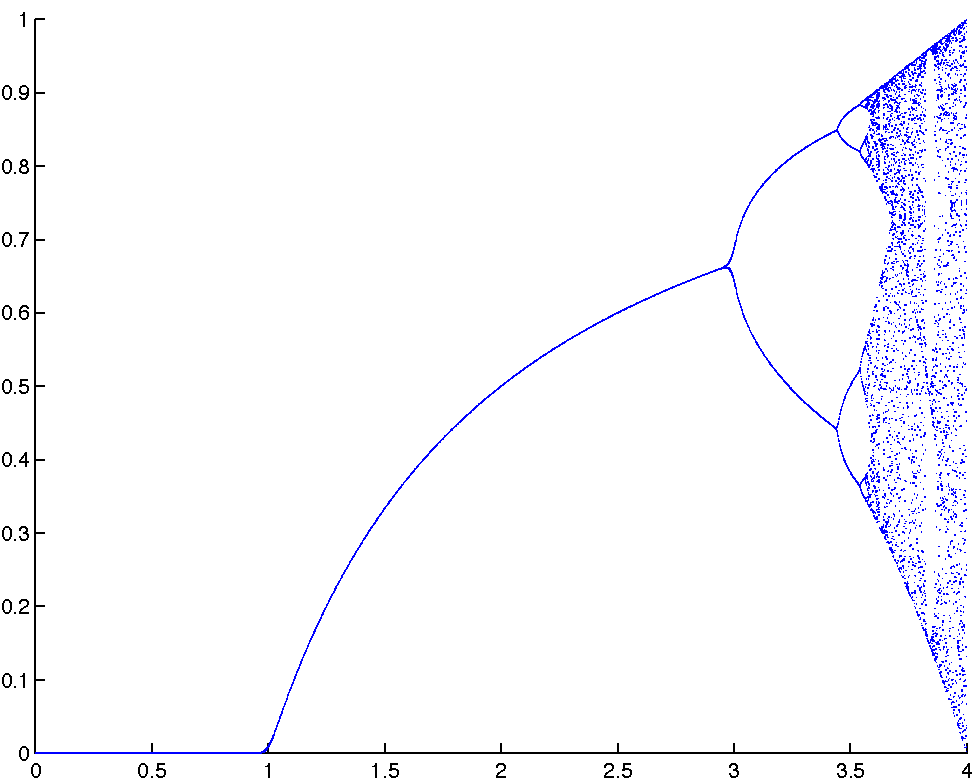
\includegraphics[scale=0.55]{plot_A01_P01.pdf}
    \caption{Logistic Map Bifurcation Diagram}
	\label{fig:plot_logistic_map_bifgraph}
\end{figure}


\setcounter{chapter}{2}
\setcounter{section}{0}
\section{Problem 2: Logistic growth in continuous time}
We have to solve the equation
\begin{equation}
\frac{dx}{dt} = rx (1-\frac{x}{K})  = r(x - \frac{x^2}{K}) = \frac{rx(K-x)}{K}
\label{eq:p02_main}
\end{equation}
using the separation of variables
\begin{equation}
\frac{K}{x(K-x)}dx = rdt
\end{equation}
decomposing the right part with partial fractions
\begin{equation}
\frac{K}{x(K-x)}=\frac{A}{x} + \frac{B}{K-x}
\end{equation}
We find A and B
\begin{align}
A&= \frac{K - Bx}{K-x} \\
B &= \frac{K-A(K-x)}{x}
\end{align}
Supposing $A = 1$, and according to above, $B$ is also equal to $1$, so our partial fraction decomposition is
\begin{equation}
\frac{K}{x(K-x)}=\frac{1}{x} + \frac{1}{K-x}
\end{equation}
Now we have to take the integral from both parts:
\begin{align}
\int{\frac{1}{x}+\frac{1}{K-x}dx} &= \int{rdt}\\
\int{\frac{1}{x}}+\int{\frac{1}{K-x}dx} &= r\int{dt}\\
\ln{x} - \ln{K-x} &= rt + x_0\\
\ln{\frac{x}{K-x}} &= rt + x_0\\
\frac{x}{K-x} &= x_0e^{rt}
\end{align}
Finally the solution 
\begin{equation}
x(t) = x_0Ke^{rt}\frac{1}{K + x_0(e^{rt}-1)}
\end{equation}

\subsection{Determining the stability of equilibria}

To determine the stability of the two equilibria points found solving the equation \ref{eq:p02_main} in $0$
\begin{align}
x_1 &= 0\\
x_2 &= K
\end{align}
one has to derive it for $x$:
\begin{equation}
f' = - r(\frac{x}{K} - 1) - \frac{rx}{K}\\
\label{eq:p02_diffmain}
\end{equation}
Substituting $x_1$ and $x_2$ into \ref{eq:p02_diffmain} yields:
\begin{align}
f'(x_1) &= -1 \\
f'(x_2) &= -r
\end{align}

One finds that if $ f'(x_1) $ with $x_1 = 0$, then $x^{\ast}$ is always stable, while if $ for r < 0 \rightarrow f'(x_2) > 0 $ with $x_2 = -r $ $x^{\ast}$ is repelling.



\setcounter{chapter}{3}
\setcounter{section}{0}
\section{Problem 3: Hardy-Weinberg equilibrium}
Assuming HWE fot three alleles (allele and genotype frequences):

\[  (A+B+0)^2 = A^2 + B^2 + 0^2 + 2AB + 2A0 + 2B0 = 1  \]

We could solve the equation: 

\[  (A+B+0)^2 = (p+q+r)^2 = p^2 + q^2 + r^2 + 2pq + 2pr + 2qr = 1  \]

And given observable genotype frequences
\begin{align}
0^2 &= \frac{900}{10000} = 0.09 = r^2 \rightarrow r = 0.3 \\
2AB &= \frac{2000}{10000} = 0.20 = 2pq \rightarrow pq = 0.1 \\
A^2 + 2A0 &= \frac{1600}{10000} = 0.16 = p^2 + 2pr\\
\\
p^2+2*0.3*p &= 0.16 \\
p_1 &= \frac{1}{5} \\
p_2 &= -\frac{4}{5} \text{~not acceptable}\\
\\
q = \frac{0.1}{0.2} = 0.5
\end{align}

So, the frequency for $B$ allele is equal to $0.5$

\subsection{HW Equilibrium}

\begin{align}
A^2 &= \frac{1500}{10000} = 0.15 = p^2 \rightarrow p = 0.39 
\end{align}
\begin{center}
\begin{tabular}{|l|l|l|}
\hline genotype & expected & observed \\ 
\hline PP & 10000*0.04 = 400 & 1500 \\ 
\hline 
\end{tabular} 
\end{center}

Hence, assuming population carrying $AA$ is $1500$, we are not at the equilibrium of HW $(p^{2}_b = 0.15 \neq p^{2}_a = 0.04)$

\setcounter{chapter}{4}
\setcounter{section}{0}
\section{Problem 4: Sequence alphabets}

\subsection{A: Amino acid sequences}

According to the number of amino acids $c$, $c_1 = 20 \text{ standard aminoacids} | c_2 = 22 \text{ standard + non-canonical}$ we consider there are:

\begin{align}
\text{for } c_1 = 20 \text{ then } &s_{space} = c_1^L, 20^{50} = 1.13*10^{65}\\
\text{for } c_2 = 22 \text{ then } &s_{space} = c_2^L, 22^{50} = 1.32*10^{67}
\end{align}

Since each aminoacid is not codified by an unique codon (3 nt), the number of unique DNA sequences is much larger then unique aminoacids sequences.


\subsection{B: Amino acids sequences and DNA sequences}

Each amino acid is codified by $3~nt$, so for a sequence of $50$ amino acids we need $150~nt$ or $153~nt$ if we consider the codon stop at the end of the codifying sequence.

\begin{align}
\text{for } L = 150 \text{ then } &d_{space} = c^L =  4^{150} = 2.04*10^{90}\\
\text{for } L = 153 \text{ then } &d_{space} = c^L =  4^{153} = 1.30*10^{92}
\end{align}

\setcounter{chapter}{5}
\setcounter{section}{0}
\section{Problem 5: Random sequences}

\subsection{a: Average and Expected distance}

If the Hamming distance is the number of coordinates where two vectors $x = (x_1,\dots,x_n) $ and $y = (y_1, \dots, y_n)$ of length $N$ differ

\[  d_H(x,y) = \sum\limits_{i=1}^{n} | x_i -y_i |\]

For a set $A \subseteq  F^{n}_{2}, |A|$ denotes the cardinality of $A$. The average distance in A is defined by 

\begin{equation}
dist(A) = \frac{1}{|A|^2}\sum\limits_{x\in A}\sum\limits_{y\in A} d_H(x,y)
\end{equation}

Hence 

\begin{equation}
dist(F^{n}_{2}) = \frac{1}{2^{2n}}\sum\limits_{x\in F^{n}_{2}}\sum\limits_{y\in F^{n}_{2}} d_H(x,y) = \frac{n2^{n-1}2^n}{2^{2n}} = \frac{n}{2}
\end{equation}

Let $V$ be some finite set with $q$ elements where $n \geq 1$ and $V^n$ is the dimension of sequence space.  $P$ is the common probability distribution. Then, we have

\[  \frac{n(q-1)}{q} - L(P) \leq Ed_H(X,Y) \leq \frac{n(q-1)}{q} \]

where $L(P)$ measures how skewly $P$ is distributed as

\[  L(P) = q^{n-1} \sum\limits_{x \in V^n} \left[P(x)-\frac{1}{q^n}\right]^2 \]

If $ 2\leq q \geq 4$, (in DNA $q=4$) then 

\[  Dd_H(X,Y) \leq )\frac{n(q-1)}{q^2} + \frac{2}{q}L(P) \]

Hence

\[  \frac{n(q-1)}{q^2}  \leq Ed_H(X,Y) \leq \frac{n(q-1)}{q^2} + \frac{2}{q}L(P) \]

This gives out that for two i.i.d. random sequences with the common probability distribution $P$, we have for  $n = L$ and $q = 4$
\begin{equation}
Ed_H(X,Y)  = \frac{n(q-1)}{q} = \frac{L(4-1)}{4} = \frac{3}{4}L
\end{equation}


\subsection{b: Number of sequences at a certain distance}

For a binary sequence, it is a composition of $n$ elements in $L$ places at distance $1$

\[  \frac{L!}{(L-1)!} \]

It is a composition of $n$ elements in $L$ places for $K$ differences:

\[  \frac{L!}{(L-K)!} \]

For DNA sequences:


could be a permutation with repetitions?

\subsection{c: Replication of sequences}
\begin{equation}
q_{ij} = p^{H_{ij}}(1-p)^{L-H_{ij}}
\end{equation}
\setcounter{chapter}{6}
\setcounter{section}{0}
\section{Problem 6: Quasispecies}

\[ \frac{dx}{dt} = wx - \varPhi x \] 
\[ w = (w_{ij}) = (f_{j}q_{ji}) = \begin{bmatrix}
       0 & q_{10}\\[0.3em]
       f_0q_{01} & 0 \\[0.3em]
     \end{bmatrix} \] 
     
In the limiting case of completely error-free replication, $Q$ becomes the identity matrix: all diagonal entries are one, all off-diagonal entries are zero. In our case the replication is error free with probability $q$.


\[ \text{with } f_1 = 1 \text{ and } f_0 > 1 \rightarrow w = \begin{bmatrix}
       0 & q\\[0.3em]
       fq & 0 \\[0.3em]
     \end{bmatrix} \] 
 
$\varPhi$ is the largest eigen value of $w$, while $x$ is the eigen vector of $w$.

To find eigen values and eigen vector: $ |w - \lambda I | = 0 $ 

\[ \begin{bmatrix}
       -\lambda & q\\[0.3em]
       fq & -\lambda \\[0.3em]
     \end{bmatrix} = 0 \rightarrow \lambda^2 - fq^2 = 0 \rightarrow \left\{ \begin{array}{l}
         \lambda_1 = +q\sqrt{f}\\
         \lambda_2 = -q\sqrt{f}\\
       \end{array} \right. \] 

$\varPhi$ is the largest eigen value of $w \rightarrow \varPhi = \lambda_1 = q\sqrt{f}.$

\[ \begin{pmatrix}
       x'_0 \\[0.3em]
       x'_1 \\[0.3em]
     \end{pmatrix}  = \begin{pmatrix}
            0 & q \\[0.3em]
            fq & 0 \\[0.3em]
          \end{pmatrix}\begin{pmatrix}
                 x_0 \\[0.3em]
                 x_1 \\[0.3em]
               \end{pmatrix} - q\sqrt{f}\begin{pmatrix}
                      x_0 \\[0.3em]
                      x_1 \\[0.3em]
                    \end{pmatrix} \rightarrow \begin{pmatrix}
                           x'_0 \\[0.3em]
                           x'_1 \\[0.3em]
                         \end{pmatrix}  = \begin{pmatrix}
                                qx_1\\[0.3em]
                                fqx_0\\[0.3em]
                              \end{pmatrix} + \begin{pmatrix}
                                     -q\sqrt{f}x_0 \\[0.3em]
                                     -q\sqrt{f}x_1 \\[0.3em]
                                   \end{pmatrix} = 
                                   \begin{pmatrix}
                                    qx_1 -q\sqrt{f}x_0 \\[0.3em]
                                    fqx_0 -q\sqrt{f}x_1 \\[0.3em]
                                     \end{pmatrix}
                                   \] 

\begin{align}
x'_0 &= qx_1 - q\sqrt{f}x_0 = f(x_0, x_1 ) \\
x'_1 &= fqx_0 - q\sqrt{f}x_1 = g(x_0, x_1)
\end{align}

To find the equilibrium points $f(x_0, x_1) = g(x_0, x_1) = 0$ 

\[\left\{ \begin{array}{l}
         x^*_0 = \frac{1}{\sqrt{f}}x^*_1\\
         x^*_0 = \frac{\sqrt{f}}{f}x^*_1 = \frac{1}{\sqrt{f}}x^*_1\\
       \end{array} \right. \rightarrow x^*_0 = \frac{1}{\sqrt{f}}x^*_1 \]
       
To study the  stability of equilibrium point, we can use jacobian matrix:

\[ J = \begin{bmatrix}
       \frac{\partial f}{\partial x_0} & \frac{\partial f}{\partial x_1} \\[0.8em]
       \frac{\partial g}{\partial x_0} & \frac{\partial g}{\partial x_1}\\[0.8em]
     \end{bmatrix} = \begin{bmatrix}
            -q\sqrt{f} & q \\[0.3em]
            fq & -q\sqrt{f}\\[0.3em]
          \end{bmatrix} 
\]

For stability we need negative eigen value from jacobian matrix:

\[ |J-\lambda I] = 0 \rightarrow \left\{ \begin{array}{l} tr(J) < 0 \\ det(J) > 0 \end{array} \right. \]

\[ tr(J) = -q\sqrt{f} -q\sqrt{f} = -2q\sqrt{f} < 0 \]
\[ det(J) = (-q\sqrt{f})*(-q\sqrt{f}) -fq^2 = fq^2 -fq^2 = 0 \]
From the determinant of J matrix we can not conclude any result about stability of steady states.

\subsection{c}

\[ \textbf{If } f_0 = f_1 = 1 \rightarrow x^*_0 = x^*_1 \rightarrow \text{population genotipe 0 and 1 is the same in whole population at steady state.}  \]

\subsection{d}

\[ \textbf{If } f_0 \gg 1 \rightarrow x^*_1 = \sqrt{f}x_0 \]
\[ \left\{ \begin{array}{l}
         x_0 \text{ goes extinct}\\
         x_1 = \infty \rightarrow \text{ whole population is type 1}\\
       \end{array} \right. \]
